\subsubsection{Convolutional Layer}
\label{sec:cnn-convolutional-layer}
The first convolutional layer in a network usually works directly on the prepared input data for finding features.
As the name suggests it performs a convolution with a filter matrix of arbitrary size on an input matrix of arbitrary size.
The input matrix corresponds to spatial input neurons and is, for example, an image $\vec{I} \in \mathbb{R}^{u \times v}$.
The filter or kernel matrix $\vec{K} \in \mathbb{R}^{i \times j}$ contains $i \cdot j$ weights of the network.
The filter is moved across the neurons and performs a dot product within its window.
Hence, its weights are reused for different areas in the image.
\figref{fig:convolution} illustrates the following operation.
In reference to the figure, the kernel covers the four elements in the top right corner of the input image.
Hence, the dot product multiplication for this setup yields $5 \cdot 1+4 \cdot (-1)+1 \cdot (-1)+3 \cdot 1=3$.
This result is stored in a new matrix $\vec{F}$ at its corresponding place.
In the end, this matrix will hold all values of the convolution operation.
After each calculation of the dot product, the filter matrix moves.
The corresponding step size is called stride.
A stride of $s=1$ moves the filter by one pixel or neuron, respectively.
There can be a different stride along the row and height dimension.
This resulting matrix is called a feature map because it stores the features extracted from the input.
With
\begin{subequations}
	\label{eq:feature-map-shape}
	\begin{align}
		\dim(\vec{F})_1 &= \floor \left( \frac{u - i}{s}+1 \right) \\
		\dim(\vec{F})_2 &= \floor \left( \frac{v - j}{s}+1 \right)
	\end{align}
\end{subequations}
its shape can be calculated.
\begin{figure}
	\centering
	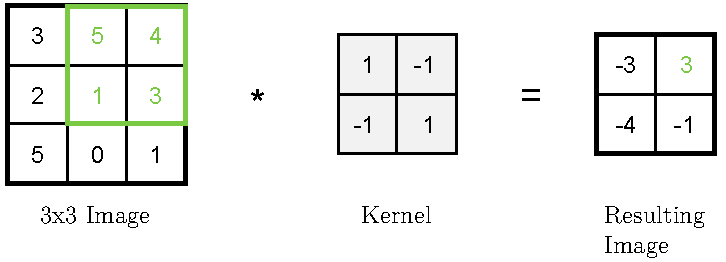
\includegraphics{images/convolution.pdf}
	\caption[Convolution of an image with a kernel]{Convolution of an image $\vec{I}$ with a kernel $\vec{K}$. The $2 \times 2$ kernel is moved across the $3 \times 3$ image and performs a dot product multiplication within its window each time. Here, the kernel moves with a stride of $s=1$, which results in the shown image on the right, the so-called feature map $\vec{F}$.}
	\label{fig:convolution}
\end{figure}
In this operation, the feature map is always smaller than the input, because only convolutions are performed with the filter inside the input.
Sometimes this is not desirable, as it can lead to loss in information in the edge regions.
This is because they are less frequent inside the filter window.
Moreover, if multiple convolutions are performed consecutively, the feature map constantly shrinks, because each convolution operates on the latest feature map, until no feature can be extracted anymore or only few detailed ones.
\begin{figure}
	\centering
	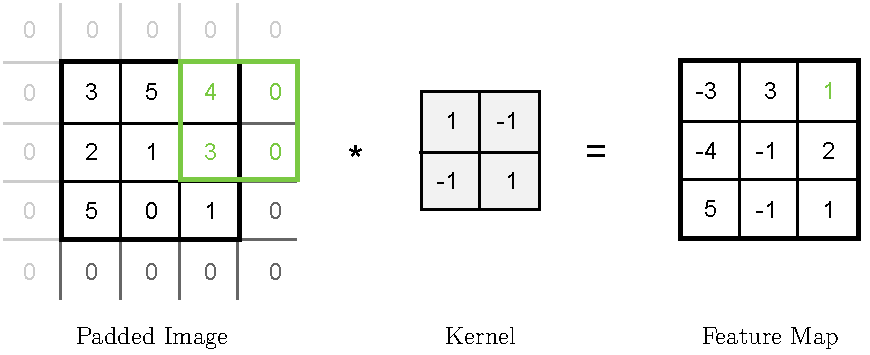
\includegraphics{images/convolution_padding.pdf}
	\caption[Convolution of a padded image with a kernel]{Convolution of a padded image with a $2 \times 2$ kernel $\vec{K}$. The $3 \times 3$ image $\vec{I}$ is surrounded with $p=0.5$ rounds of zeros for yielding a feature map $\vec{F}$ of same size. If the amount of padding is odd, two contiguous sides are preferred.}
	\label{fig:convolution-padding}
\end{figure}
In practical terms, there are two common conventions for convolutions, which are called valid and same in the following.
The former defines that no padding is applied and therefore a valid convolution is performed because only the real input and full kernel windows are taken into account.
This means that the feature map has a size of $\vec{F} \in \mathbb{R}^{\dim(\vec{F})_1 \times \dim(\vec{F})_2}$.
The latter means, that the size of the feature map equals the one of the input.
Thus, a padding $p$ can be applied to the input.
This means surrounding the input with zeros to create a larger input.
The convolution operates like usual, just on a larger input.
How much padding $p$ needs to be applied can be calculated by comparing both matrix shapes.
Therefore, the expression
\begin{subequations}
	\begin{equation}
		u := \frac{u-i+2p}{s}+1
	\end{equation}
needs to be valid, yielding
\begin{equation}
	p = \frac{u(s-1)+i-s}{2}
\end{equation}
\end{subequations}
for calculating the amount of padding on each related side.
However, in general, this only covers the padding height.
If the image or filter are not symmetric, the padding along the width needs to be calculated as well by replacing $u$ with $v$ and $i$ with $j$.
%Another remark is, that in computer vision filter sizes usually are odd.
%There can be two reasons for this.
%First, the filter has a center which helps to tell where exactly the filter points to.
%Second, the padding $p$ is even.
If the amount of padding is odd, it is performed in half rounds around the image where two contiguous sides of the image are preferred like it is shown in \figref{fig:convolution-padding} with the help of transparency.
Only the padding at the right and at the bottom are taken into account for creating a filter matrix with the same shape of the original input.
For three-dimensional inputs, where each matrix along the depth dimension is called channel, a convolution is performed almost identically.
Instead of a kernel with a depth of one as for a two-dimensional input, it is extended to a depth that matches the input yielding $\dim\left(\vec{K}\right)_3 = \dim\left(\vec{I}\right)_3$.
Then a common dot product multiplication is calculated for every input channel with its corresponding filter channel.
This results in a matrix with the depth of the input and filter.
Finally, the resulting depth channels are summed up element-wise which results in a matrix with depth one, i.e. $\dim\left(\vec{F}\right)_3 = 1$.
For the case of an RGB image, that is an image with three channels representing the colors red, green and blue, a filter would have a depth of three and a final convolution result would always have a depth of one.
This example is illustrated in \figref{fig:convolution-channels}.
\begin{figure}
	\centering
	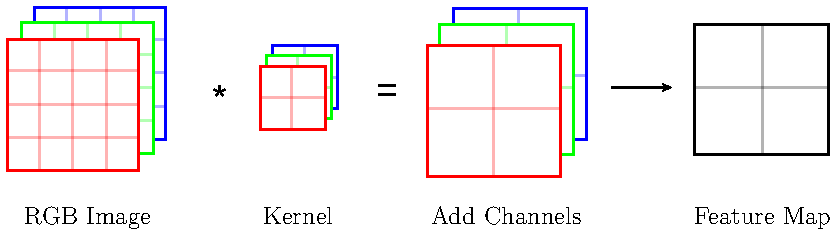
\includegraphics{images/convolution_channel.pdf}
	\caption[Convolution of input with multiple channels]{Convolving an RGB input $\vec{I}$ with $\dim(\vec{I})_3=3$ channels needs a kernel $\vec{K}$ with $\dim(\vec{K})_3 = \dim(\vec{I})_3$. This results in one convolution result per corresponding channels. Those are summed element-wise for yielding a two-dimensional feature map $\vec{F}$.}
	\label{fig:convolution-channels}
\end{figure}
Usually, at the end of a convolutional layer, a bias addition is performed for simulating the neurobiological spike of a neuron.
This result is put into an activation function like the ones from \figref{fig:activation-functions}.
Both the methods and their purposes are analog to the ones known from multilayer perceptron networks.

The kernel in \figref{fig:convolution} would find top-left to bottom-right diagonal lines because its convolution result is higher if the pixels in its window represent such a shape.
For example, there is a black image with white shapes.
If the filter is on a plain surface, where all pixel values have the same intensity, the convolution result is 0 due to the positive and negative weights.
However, if it is over such a line, the result is higher because the pixels representing the line are fully taken into account.
If the line points into the other direction the representing pixels are not taken into account, while the other two are weighted negatively.
Like this but with slightly larger kernels and different weights more complex features can be found.
Finding discriminative features depends on a satisfiable set of weights and biases, though.
It is also possible to perform multiple different convolutions on the same input to find different features.
They are stored as a matrix, where the number of different features represents the depth of the feature map $\vec{F}$.
This whole process solves the limitation to a fixed position of features of the multilayer perceptrons architecture.
Even if, for example, a digit is not centered anymore in the image, all features are found, because the kernel is moved over the image for checking the presence of a certain feature.
Hence, this keeps the spatial relationship of pixels that is lost if an input is flattened as with multilayer-perceptrons networks, where each perceptron is responsible for one single pixel.
Furthermore, because each feature is found by a moving filter, convolutional neural networks need way fewer weights and biases due to the possibility of reusing them for different image areas.
The accuracy compared to multilayer perceptron networks is improved by concatenating several convolutions.
That means a convolution is performed on the activation of an earlier convolution or more generally on the activation of its preceding layer.
This way, first, rough features like edges are found for narrowing down possible classes, and the deeper it gets into the network, the finer the features get.